\chapter{Аналитический раздел}
\label{cha:analysis}
\section{Цель и задачи работы}

\section{TCMalloc}
TCMalloc это аллокатор памяти, разработанный компанией Google и являющейся заменой стандартному системному аллокатору, он имеет следующие характеристики:
\begin{itemize}
	\item Быстрое выделение и освобождение памяти для большинста объектов. Обекты кэшируются в зависимости от режима, либо кэш в каждом потоке, либо кэш на логический процессор. Большинство аллокаций не требуют синхронизации доступа к ресурсам, благодаря этому конкуренция за выделение памяти сводится к минимуму и обеспечивает хорошее масштабирование для многопоточных приложений.
	\item Гибкое использование памяти, освобожденная память может быть переиспользована для объектов различных размеров или возвращена системе.
	\item Низкие накладные расходы на память под каждый объект за счет выделения ``страниц'' объектов одинакового размера. Что приводит к пространственно-эффективному представлению небольших объектов.
	\item Низкая стоимость сэмлирования, которое позволяет получить детальное представление об использовании памяти приложений.
\end{itemize}

\subsection{Общее представление}

\begin{figure}[!h]
	\begin{center}
		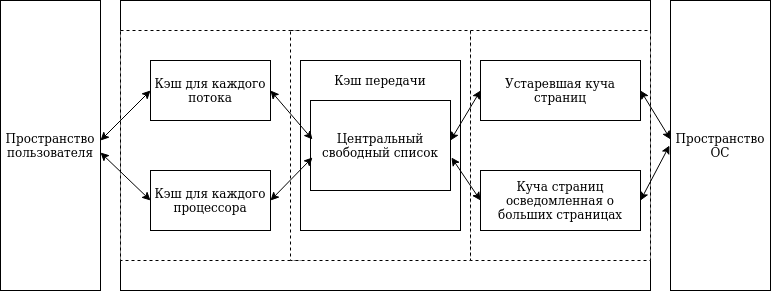
\includegraphics[scale=0.6]{images/tcmalloc-overview.png}
		\caption{Внутренняя структура TCMalloc.}
		\label{tcmalloc-overview}
	\end{center}
\end{figure}

Библиотеку TCMalloc можно разбить на 3 основных компонента. Фронт-энд, миддл-энд и бэк-энд:
\begin{itemize}
	\item Фронт-энд является кэшом, который предоставляет быстрое выделение и освобождение памяти приложению.
	\item Миддл-энд отвечает за наполнение фронт-эгд кэшей.
	\item Бэк-энд управляет памятью, которая выделяется приложению самой ОС.
\end{itemize}

Фронт-энд может использоваться как в режиме кэш на каждый поток, так и в режиме кжш на каждый логический процессор. Бэк-энд поддерживает работу с кучей, которая осведомлена о больших страницах.

\subsection{TCMalloc фронт-энд}

Фронт-энд обрабатывает запрос на выделение памяти определенного размера. У него имеется кэш памяти, который может использоваться для выделения или хранения свободной памяти. Этот кэш доступен только одному потоку одновременно, поэтому никаких блокировок не требуется и большинство выделений и освобождений памяти выполняются быстро.

Фронт-энд удовлетворит любой запрос, если у него есть закэшированная память соответствующего размера. Если кэш для этого конкретного размера пуст, будет сделан запрос на пополнение кэша в миддл-энд, который включает в себя центральный список свободной памяти и кэш передачи.

Если миддл-энд исчерпан или если запрошенный размер больше максимального размера, который кэшируется фронт-эндом, запрос будет отправлен бек-энду, чтобы либо удовлетворить большое выделение памяти, либо пополнить кэш в миддл-энде. Бэк-энд также называется кучей страниц.

На данный момент существует 2 реализации фронт-энда:
\begin{itemize}
	\item Первоначально он поддерживал кэширование объектов по каждому потоку (отсюда и название Thread Caching Malloc). Однако это привело к появлению областей памяти, которые масштабировались с увеличением количества потоков. Современные приложения могут иметь большое количество потоков, что приводит либо к большим объемам совокупной памяти для каждого потока, либо к тому, что многие потоки имеют крошечные кэши для каждого потока.
	\item Совсем недавно TCMalloc начал поддерживать режим кэширования под каждый логический процессор. В этом режиме каждый логический процессор в системе имеет свой собственный кэш, из которого выделяется память. Примечание: На x86 логический процессор эквивалентен гиперпотоку.
\end{itemize}

Различия между режимами кэшами по потокам и процессорам полностью ограничиваются реализациями malloc/new и free/delete.

\subsection{Выделение памяти под большие и маленькие объекты}

Размер на выделение памяти под малые объекты сопоставляется c одним из 60-80 распределяемых размерных классов. Например, выделение 12 байт будет округлено до 16-байтового класса размера. Размерные классы предназначены для минимизации объема памяти, который тратится впустую при округлении до следующего по величине размерного класса.

При компиляции с  \_\_STD CPP\_DEFAULT\_NEW\_ALIGNMENT\_\_ <= 8 используется набор размеров, выровненных по 8 байтам. Это меньшее выравнивание сводит к минимуму потери памяти для многих распространенных размеров распределения (24, 40 и т.д.), Которые в противном случае округляются до кратного 16 байтам. Во многих компиляторах это поведение контролируется флагом \textbf{\textit{-fnew-alignment=...}}. Когда \_\_STD CPP\_DEFAULT\_NEW\_ALIGNMENT\_\_ не указан (или больше 8 байт), использются стандартные 16-байтовые выравнивания для \textit{\textbf{::operator new}}. Однако при выделении менее 16 байт может быть возвращен объект с меньшим выравниванием, так как ни один объект с большим требованием выравнивания не может быть выделен в пространстве.

Когда запрашивается объект заданного размера, этот запрос сопоставляется с запросом определенного класса размера с помощью функции \textit{\textbf{SizeMap::GetSizeClass()}}, и возвращаемая память принадлежит этому классу размера. Это означает, что возвращаемая память по крайней мере так же велика, как и запрошенный размер. Выделения памяти из размерных классов обрабатываются фронт-эндом.

Объекты размером больше предела, определенного максимальным размером (\textbf{kMaxSize}), выделяются непосредственно из бэкэнда. Как таковые они не кэшируются ни фронт ни миддл эндами. Запросы на выделение больших размеров объектов округляются до размера страницы TCMalloc.

\subsection{Освобождение памяти}

Когда объект освобождается, компилятор предоставляет размер объекта, если он известен во время компиляции. Если размер не известен, он будет найден на карте страницы. Если объект мал, он будет помещен обратно в кэш фронт-энда. Если объект больше \textbf{kMaxSize}, он возвращается непосредственно в кучу страниц.